\documentclass[tikz]{standalone}

\usepackage{fontspec}

\usetikzlibrary{arrows}
\usetikzlibrary{calc}
\usetikzlibrary{decorations.pathreplacing}
\usetikzlibrary{positioning}
\usetikzlibrary{matrix}

\usepackage{fontspec}

\begin{document}

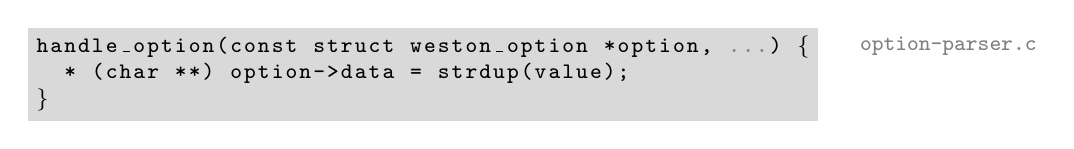
\begin{tikzpicture}
  [node distance=5mm, >=stealth',
  every node/.style={font=\footnotesize},
  every matrix/.style={fill=black!15, inner sep=1mm, row sep=0.5mm,
                        matrix of nodes, nodes in empty cells,
                        minimum height=0.5em, minimum width=.5em,
                        nodes={anchor=base, inner sep=0, font=\ttfamily\footnotesize}}]

  \matrix (snippet) {
h & a & n & d & l & e & \_ & o & p & t & i & o & n & ( & c & o & n & s & t &   & s & t & r & u & c & t &   & w & e & s & t & o & n & \_ & o & p & t & i & o & n &   & * & o & p & t & i & o & n & , &   & |[black!50]|. & |[black!50]|. & |[black!50]|. & ) &   & \{ \\
  &   & * &   & ( & c & h & a & r &   & * & * & ) &   & o & p & t & i & o & n & - & > & d & a & t & a &   & = &   & s & t & r & d & u & p & ( & v & a & l & u & e & ) & ; &   &   &   &   &   &   &   &   &   &   &   &   &   \\
\} &   &   &   &   &   &   &   &   &   &   &   &   &   &   &   &   &   &   &   &   &   &   &   &   &   &   &   &   &   &   &   &   &   &   &   &   &   &   &   &   &   &   &   &   &   &   &   &   &   &   &   &   &   &   &   \\
  };

  \node [above, anchor=west, black!50, xshift=0.5cm]
        at (snippet-1-56.east)
        {\texttt{option-parser.c}};

\end{tikzpicture}

\end{document}
